\documentclass[11pt]{article}

% package to include images
\usepackage{graphicx}

% parameters for \maketitle
\title{Computational Vision Lab 02 - Edges and Contours}
\author{Johannes Heidecke}

% paragraph formatting
\setlength{\parindent}{2em}
\setlength{\parskip}{2em}
\renewcommand{\baselinestretch}{1.1}

% prevent orphans and widows
\widowpenalty10000
\clubpenalty10000

\begin{document}

\maketitle


\section*{Exercise 1:}


XX general text XX (answer question 1)

XX Sobel: This method finds edges using the Sobel approximation to the derivative. It returns edges at those points where the gradient of I is maximum. Returns all edges that are stronger than threshold

XX t can be estimated automatically, for example simply using the default Sobel mode results in a t of 0.3715 for this image. Manual experiments with changing the value of t result in much better results for t = 0.1. There are many possible t values in the range 0.05 to 0.2 that yield almost same results. imabsdiff only shows a few pixel difference.

\begin{figure}[!hbt]
  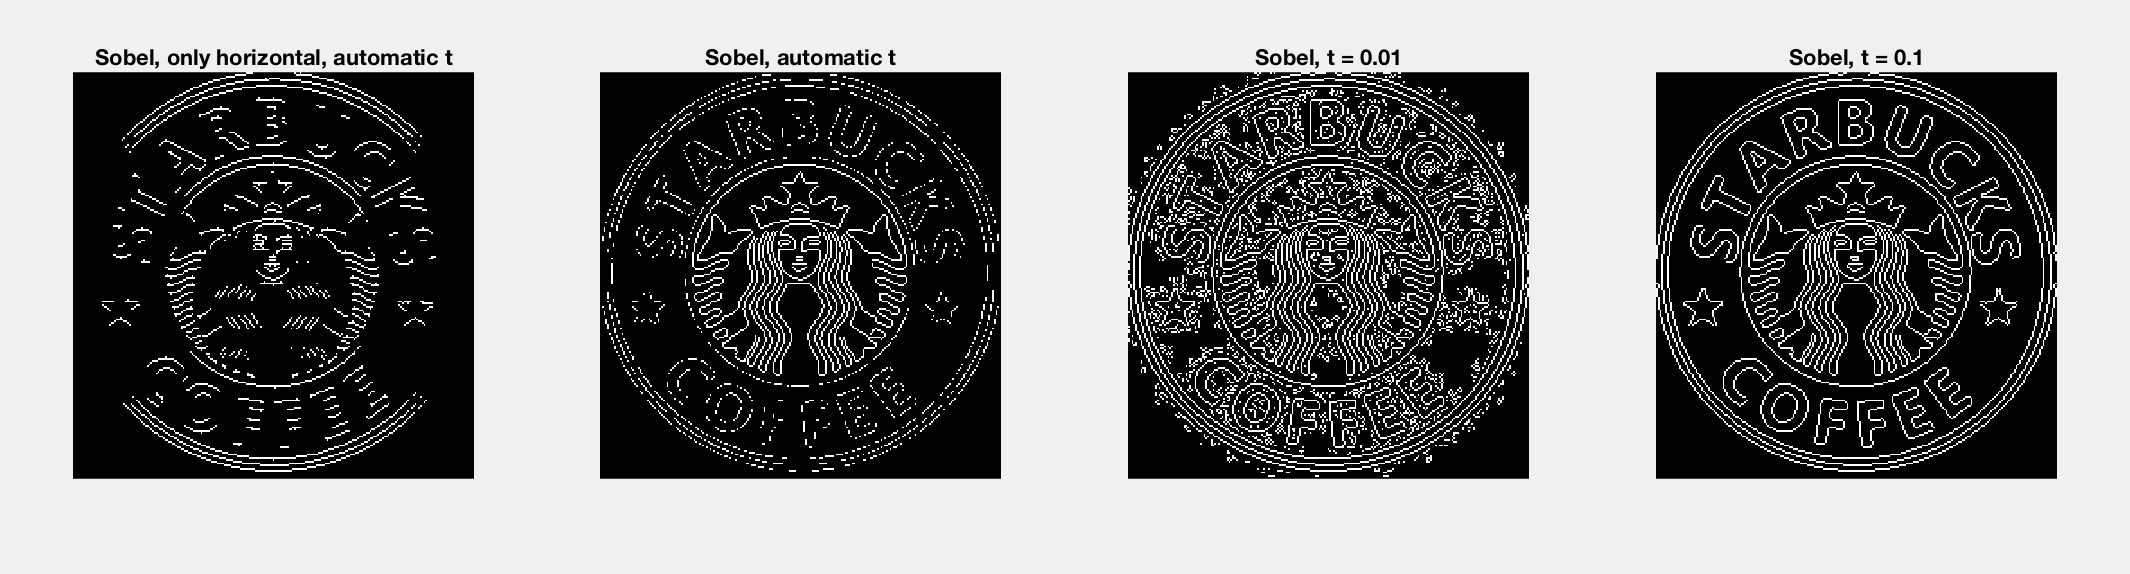
\includegraphics[width=\textwidth]{im1}
  \caption{Results with Sobel method}
  \label{fig:im1}
\end{figure}

XX Prewitt: This method finds edges using the Prewitt approximation to the derivative. It returns edges at those points where the gradient of I is maximum. Returns all edges that are stronger than threshold

XX Prewitt: automatic t is estimated at 0.3629. Much better results with a lower t of 0.25. A higher t e.g. 0.4 yields in the outer edges to not be detected anymore.

\begin{figure}[!hbt]
  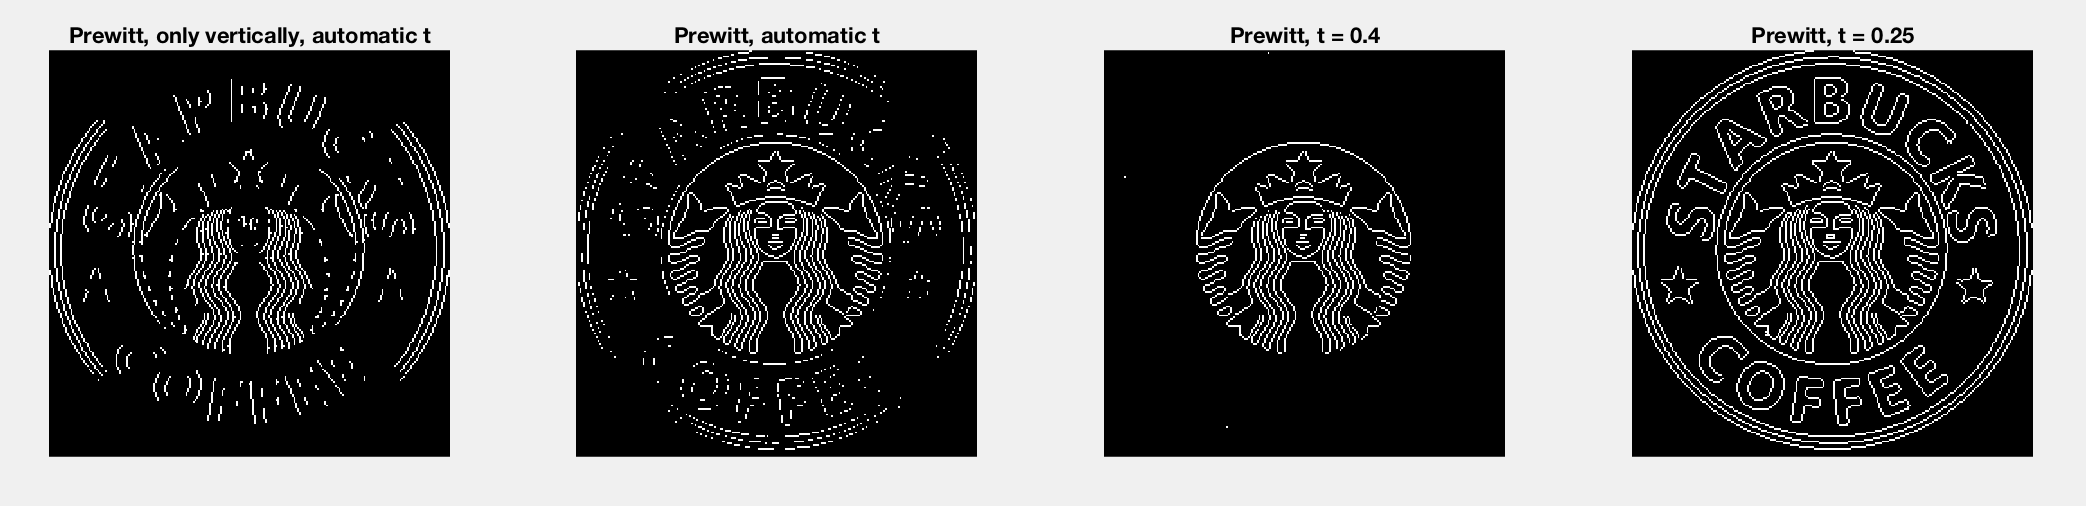
\includegraphics[width=\textwidth]{im2}
  \caption{Results with Prewitt method}
  \label{fig:im2}
\end{figure}

XX Roberts: This method finds edges using the Roberts approximation to the derivative. It returns edges at those points where the gradient of I is maximum.

XX Roberts automatic t = 0.4100

\begin{figure}[!hbt]
  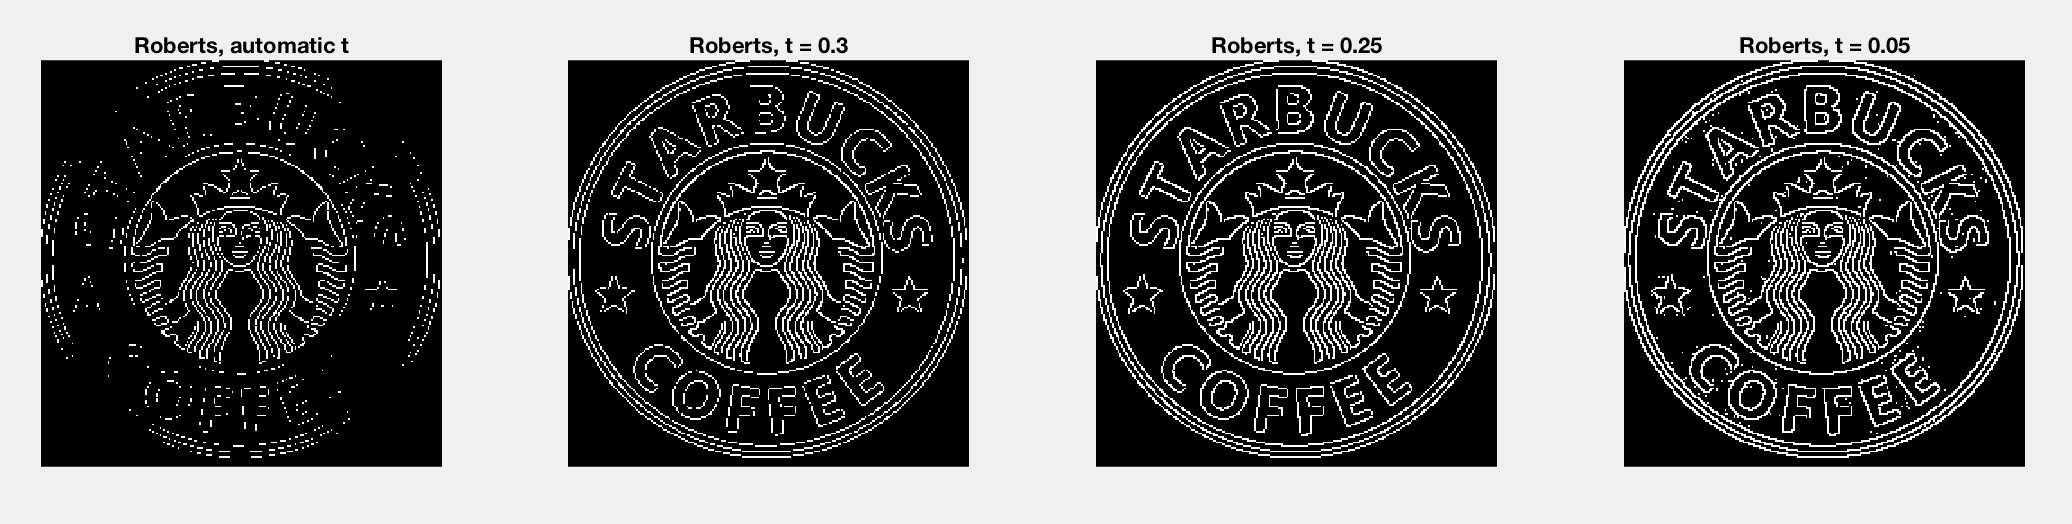
\includegraphics[width=\textwidth]{im3}
  \caption{Results with Roberts method}
  \label{fig:im3}
\end{figure}

XX log: This method finds edges by looking for zero-crossings after filtering I with a Laplacian of Gaussian filter. return all edges that are stronger than threshold.

XX automatic t: 0.022. Standard sigma is 2. Second image: change sigma to 1. Size of the gaussian filter is determined automatically as \textit{n=ceil(sigma*3)*2+1} Higher t worsens result. t can be much smaller and still yield the same results.

\begin{figure}[!hbt]
  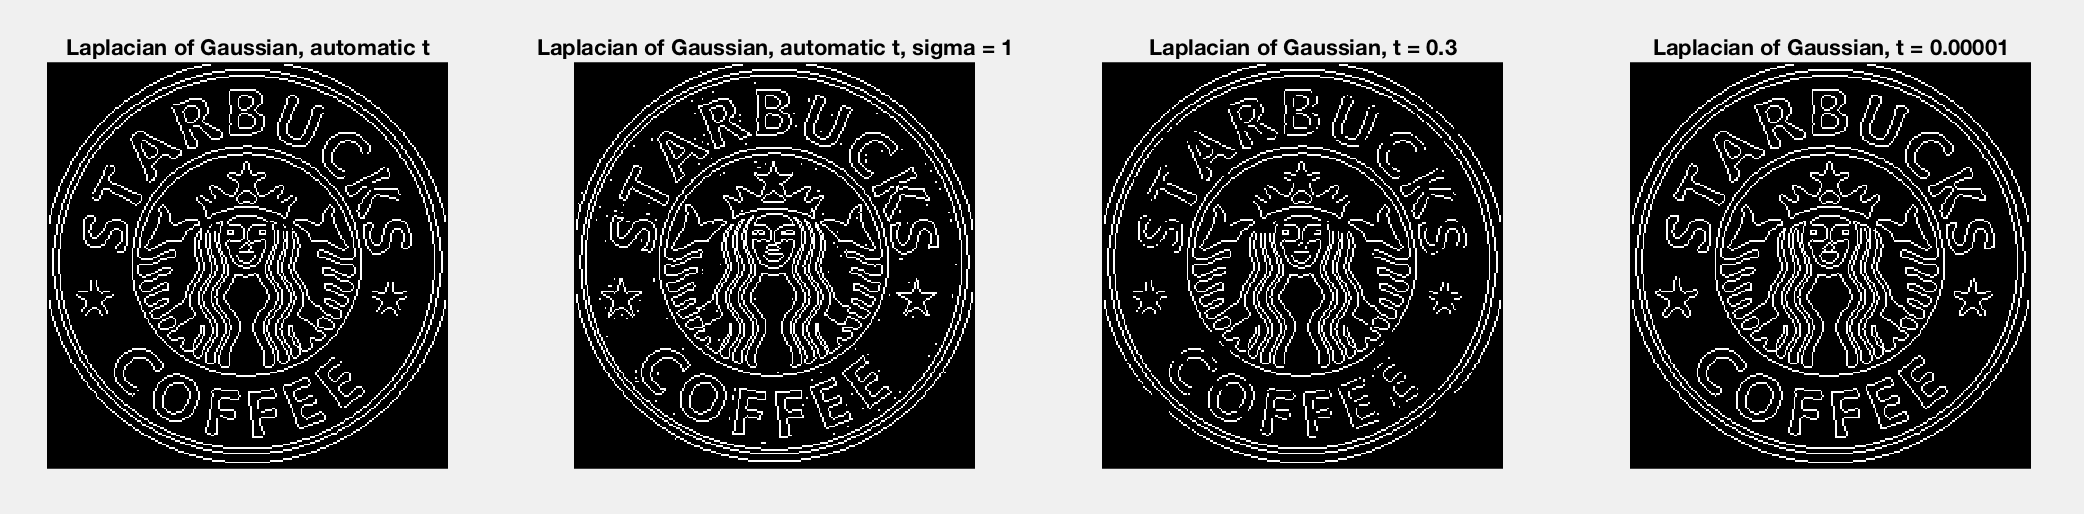
\includegraphics[width=\textwidth]{im4}
  \caption{Results with Laplacian of Gaussian}
  \label{fig:im4}
\end{figure}

XX zerocross: This method finds edges by looking for zero-crossings after filtering I with a filter that you specify, h. The edge function returns edges that are stronger than threshold.

XX for this example, after some experiments, a gaussian filter with size 5x5 and sigma 2 was chosen. The automatic t for this filter was estimated at 0.0093. Increasing this t leads to important edges not being detected anymore. Lowering the threshold produces more false positives while some edges are still not being detected. The filter adds more dimensions of complexity for determining optimal parameters. While it might be possible to accomplish very good results with the right parameters, this method seems to require a lot of manual work, since the automatic estimation of the parameters does not yield good results.

\begin{figure}[!hbt]
  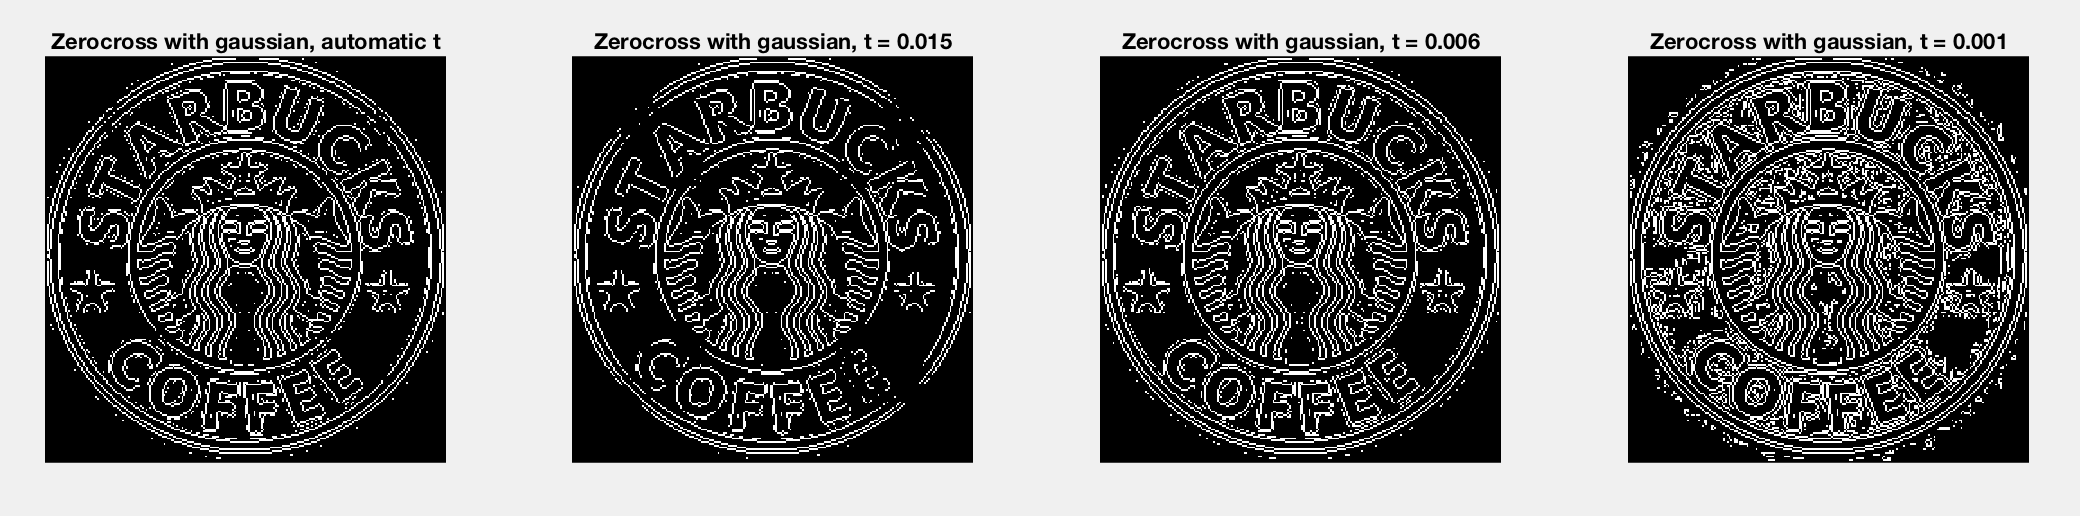
\includegraphics[width=\textwidth]{im5}
  \caption{Results with Zerocross method}
  \label{fig:im5}
\end{figure}

XX Canny: he Canny method finds edges by looking for local maxima of the gradient of I. The edge function calculates the gradient using the derivative of a Gaussian filter. This method uses two thresholds to detect strong and weak edges, including weak edges in the output if they are connected to strong edges. By using two thresholds, the Canny method is less likely than the other methods to be fooled by noise, and more likely to detect true weak edges. Disadvantage: not supported to be executed on GPU.

XX t: 0.1875    0.4688. Default: weak edge threshold is 0.4 of strong t. 

\begin{figure}[!hbt]
  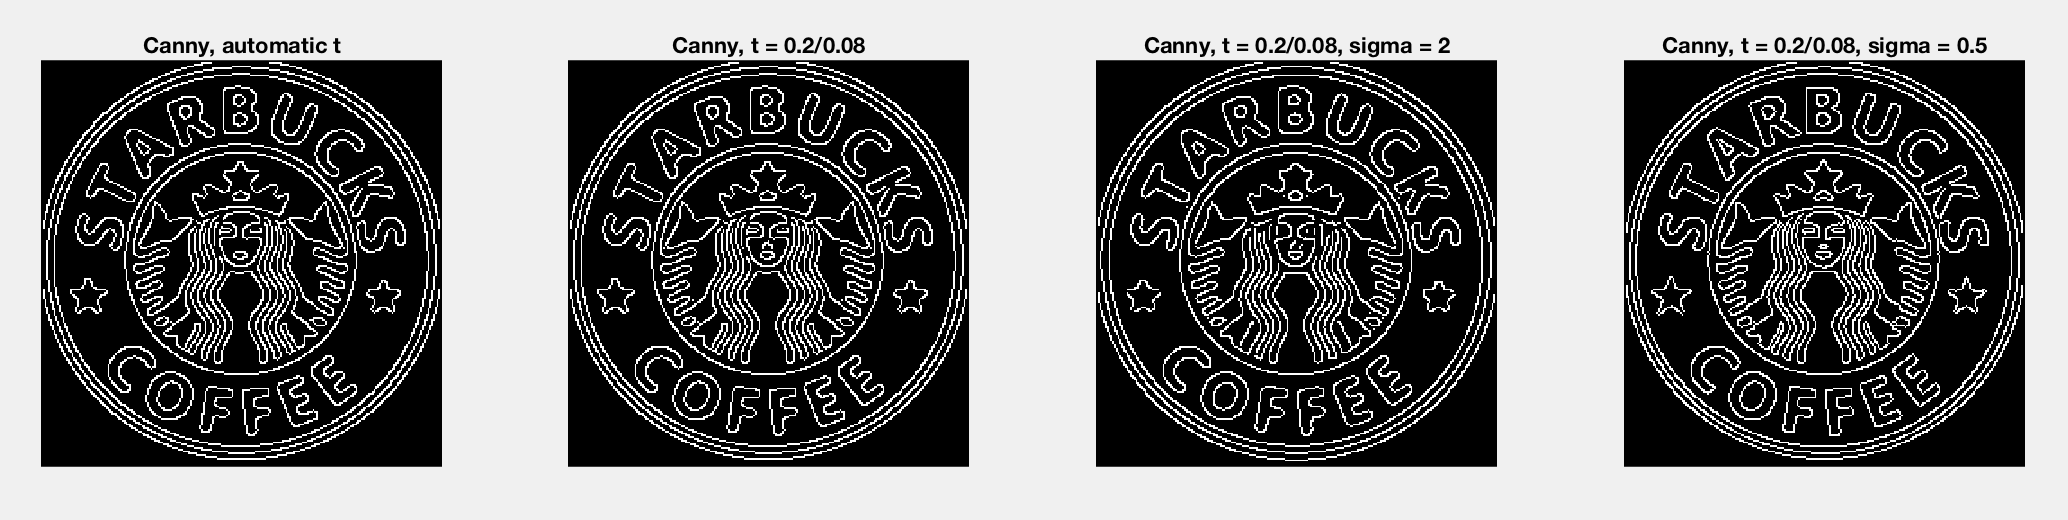
\includegraphics[width=\textwidth]{im6}
  \caption{Results with Canny method}
  \label{fig:im6}
\end{figure}

XX: answer questions 2 \& 3

XX: describe overlapping edges and images

XX: describe effects when code is run with other images, difficulties, etc.

XX answer questions 4, 5

\section*{Exercise 2:}




\end{document}